\cotefile{53}
\scanpage{23}
% loc 1–2, opening bracket
[\unsure{cel|cela|cet|ceci} exprime que l'hom $A\mathrel{\unsure{\text{---}|\to}}k'$ est un hom d'algèbres]

% loc 3–6, Si G
Si $G$ est muni d'une loi de comp. de $=$ $\mathrm{Dist}(D)$, celle-ci est ass. (comm) \unsure{sss|ssi} celle de $G$ l'est, et \deleted{\unsure{unitaire}} $G$ admet une unité bilatère ssi $\mathrm{Dist}(D)$ a une unité \deleted{\unsure{élément}} $e$ telle que $\delta(e)=e\otimes e$.

% loc 7–9, Dire que
Dire que $G$ opère sur un module $M$ \inserted{\unsure{(à g.)}} signifie que $\mathrm{Dist}(G)$ y opère à gauche -- et cette opération étend celle de $G$.

% loc 10–14, NB
\uline{NB} Dans certains cas, $\mathrm{Dist}(\unsure{X|x})$ se reconstitue à partir de $\mathrm{dist}(X,k)=\unsure{\mathrm{Dst}|\mathrm{Dist}}(X)(k)$, p.ex. si $A$ est \deleted{\unsure{de t.f.}} projectif de t.f. sur $k$, ou plus gén. si $A$ est somme de modules projectifs de t.f (p.ex. \deleted{\unsure{si}} $k$ un corps) -- mais alors il faut considérer $\mathrm{Dist}(\unsure{x|X},k)$ comme module topologique.

% loc 15–20, Re NB
\uline{Re NB} Surtout intéressant pour \unsure{monoïde}. En plus \deleted{\unsure{de|du}} \inserted{\unsure{du sous foncteur}} $G$, $\mathrm{dist}(G)$ \unsure{'} [\unsure{resp.} $\mathrm{Dist}(G,k)$] contient \unsure{toute} l'information infinitésimale de $G$ : p.ex. l'\uline{algèbre de Lie} de $G$ est \unsure{contenue|contenu} dans $\mathrm{Dist}(G\unsure{,|.}k)$, -- \deleted{\unsure{et les op.}} sa loi de $[\,]$ est induite par le crochet de l'algèbre, et en car. pos sa puiss. \unsure{pième} aussi -- de $=$ que l'hyperalgèbre.

\begin{center}\rule{1.6cm}{0.55pt}\end{center}
% loc 21, between the two rules
Cas des schémas constants : on retrouve l'\uline{algèbre} d'un groupe fini.

\begin{center}\rule{1.6cm}{0.55pt}\end{center}
% loc 22, second Cas
Cas du groupe diagonalisable
% loc 23, A = k(M)
\[
 A=k(M)\quad\text{algèbre du groupe à \unsure{coeff.|coeffs} dans } k
\]
% loc 24–25, two paired rows
\diagram{\begin{tikzcd}[ampersand replacement=\&,column sep=small,row sep=large]
 A\otimes A \arrow[r,dash] \& A \& \text{provient de} \& M\times M \arrow[r] \& M \& \text{loi de groupe}\\
 A\otimes A \& A \arrow[l] \& \text{---} \& M\times M \& M \arrow[l,swap,"\substack{\text{application}\\\text{diagonale}}"] \&
\end{tikzcd}}
% loc 26–27, lowest two lines
\[
\begin{aligned}
 &\mathrm{Dist}(\unsure{\mathbb D|D}(M)(k)=\deleted{\unsure{*}}k^{M}\quad\text{avec la loi d'\uline{algèbre} \uline{produit}}\\
 &\qquad\text{[Combinaisons \unsure{lin|lin.} infinies de \unsure{caractères}]} \qquad
 \text{(\unsure{ne dépend pas de la str. additive de|ne dépend pas de la str. d'addition de} $M$)}
\end{aligned}
\]
% archive sheet number: 22
\scanpage{24}
% loc 1, heading
$A$ algèbre d'un $k$-\deleted{groupe}\inserted{monoïde} affine $G$

% loc 2
$M$ $k$ module

% loc 3–4, opération and brace
opération de $G$ \unsure{on|en|sur} $M$ :
\[
 \text{i.e.}\quad G\longrightarrow
 \underline{\unsure{\mathrm{End}|\mathbb E\mathrm{nd}}}_{k}(M)
 =\underline{\unsure{\mathbb E\mathrm{nd}|\mathrm{End}}}_{\unsure{\mathcal O|O}}(\unsure{W|V}(M))
 \quad\overset{\deleted{\unsure{gxx|gx}}}{\vphantom{X}}
 \left\{\begin{aligned}1)&\ 1x=x\\2)&\ g(g'x)=gg'x\end{aligned}\right.
\]

% loc 5–8, Opération sans axiomes
``Opération sans axiomes'' correspond à
\[
\begin{aligned}
 &\deleted{\unsure{u:A\otimes M_{A}\to A\otimes_{k}M}}\quad
 u:M_A\mathrel{\mathop{\unsure{\text{---}|\to}}\limits_{\text{$A$ lin}}}M_A
 \qquad M_A\underset{\unsure{,|1}}{=}\tikz[baseline=(t.base)]{\node[inner sep=0pt](t){$A\otimes_k M$};\draw[thin](-.08,-.31) .. controls (.12,-.38) and (.05,.09) .. (.22,.21) .. controls (.38,.38) and (.58,.35) .. (.64,.30);}\\
 &\deleted{\unsure{Ax|M}} \\
 &\hspace{4em}\text{ou}\qquad u_0:M\longrightarrow
 \tikz[baseline=(t.base)]{\node[inner sep=0pt](t){$A\otimes_k M$};\draw[thin](-.12,-.30) .. controls (.10,-.39) and (.06,.06) .. (.25,.23) .. controls (.44,.35) and (.60,.31) .. (.64,.24);}
 \qquad\text{$k$-lin.}
\end{aligned}
\]

% loc 9, cancelled sentence
\deleted{L'axiome $1x=x$}

% loc 10–13, Si g
Si $g\in G(k')$ correspond à un hom de $k$-algèbres $A\overset{g}{\longrightarrow}k'$, alors $g_M$ sera l'endomorphisme \deleted{$\unsure{k'\otimes_A}$}\inserted{de} \tikz[baseline=(t.base)]{\node[inner sep=0pt](t){$(\deleted{\unsure{g}}k',\deleted{\unsure{k}}g)\otimes_A M$};\draw[thin](.18,-.29) .. controls (.35,-.33) and (.37,.08) .. (.50,.23) .. controls (.68,.43) and (.81,.36) .. (.81,.31);} \deleted{\unsure{défini}}\inserted{déduit} \deleted{\unsure{comme}}\inserted{de $u$} \deleted{$g\otimes_A\unsure{i}$} par changement de base, i.e. l'unique hom $M_{k'}\longrightarrow M_{k'}$ tel que le diagramme d'hom $A$-linéaires
% loc 14, bracketed fork and square
\diagram{\begin{tikzcd}[ampersand replacement=\&,column sep=2.9em,row sep=1.1em]
 \& M_A\arrow[rr,"u"]\arrow[dd,"{\tikz[baseline=(t.base)]{\node[inner sep=0pt](t){$\scriptstyle g\otimes\mathrm{id}_M$};\draw[thin](-.13,-.16) .. controls (-.06,-.19) and (-.09,.07) .. (.02,.16) .. controls (.13,.30) and (.22,.25) .. (.23,.22);}}"] \& \& M_A\arrow[dd,"{\tikz[baseline=(t.base)]{\node[inner sep=0pt](t){$\scriptstyle g\otimes\mathrm{id}_M$};\draw[thin](-.13,-.16) .. controls (-.06,-.19) and (-.09,.07) .. (.02,.16) .. controls (.13,.30) and (.22,.25) .. (.23,.22);}}"]\\
 \left[\vphantom{\dfrac{\dfrac{A}{A}}{\dfrac A A}}\right. M
 \arrow[ur]\arrow[dr] \&[-1.7em] \hspace{-2.2em}\left.\vphantom{\dfrac{\dfrac{A}{A}}{\dfrac A A}}\right] \& \& \\
 \& M_{k'}\arrow[rr,swap,"g_M"] \& \& M_{k'}
\end{tikzcd}}
% loc 15, after first diagram
est commutatif ; Mais cela signifie aussi que le diagramme
% loc 16, square
\diagram{\begin{tikzcd}[ampersand replacement=\&]
 M\arrow[r,"u_0"]\arrow[d,swap,"\mathrm{can}"] \& M\deleted{\unsure{{}_A}}\otimes A\arrow[d,"\mathrm{id}_M\otimes g"]\\
 M\deleted{\unsure{{}_k|{}_{k'}}}\otimes k'\arrow[r,swap,"g_M"] \& M\otimes k'
\end{tikzcd}}
% loc 17–19, est commutatif
est commutatif, ou encore, \unsure{notant|sachant} que la donnée de $g_M$ est équivalente à celle de $g_M^{\unsure{0|\circ}}=g_M\circ\mathrm{can}:M\mathrel{\unsure{\text{---}|\to}}M\otimes k'$, à la \deleted{\unsure{fon.}} commutativité du
% loc 20, triangle
\diagram{\begin{tikzcd}[ampersand replacement=\&]
 M\arrow[r,"u_0"]\arrow[dr,swap,"g_M^0"] \& M\otimes A\arrow[d,"\unsure{\mathrm{id}|\mathrm{Id}}_M\otimes g"]\\
 \& M\otimes k'
\end{tikzcd}}

% loc 21–22, Pour traduire
Pour traduire l'axiome 1), on fait $k'=k$, $g=\deleted{\unsure{\mathrm{id}_k|1_k}}$ $(\varepsilon:A\longrightarrow k)$, et on trouve
% loc 23, circled 1 and triangle with equation
\diagram{\begin{tikzcd}[ampersand replacement=\&,column sep=2.8em,row sep=large]
 \tikz[baseline=(t.base)]{\node[draw,circle,inner sep=1.5pt](t){$1'$};} \& M\arrow[r,"u_0"]\arrow[dr,swap,near start,"\text{---}"{sloped}] \& M\otimes A\arrow[d,"\mathrm{id}_M\otimes\varepsilon"] \& \text{comm. i.e.}\\
 \& \& M \& (\mathrm{id}_M\otimes\varepsilon)u_0=\mathrm{id}_M
\end{tikzcd}}
% archive sheet number: 23
\scanpage{25}
% loc 1–2, Pour récrire
Pour \unsure{récrire|réécrire} 2), on \deleted{écrit} prend $k'=A\otimes A$, et on choisit les deux hom
% loc 2, two parallel strokes
\diagram{\begin{tikzcd}[ampersand replacement=\&]
 \deleted{\unsure{g}} \& A^{\unsure{\cdot}}\arrow[r,dash,shift left=.55ex,"g"]\arrow[r,shift right=.55ex,swap,"g'"] \& A\otimes A \& \deleted{\unsure{g'}}\quad\text{donnés par}
\end{tikzcd}}
% loc 3, definitions
\[
 g(\lambda)=\lambda\otimes1,\quad g'(\lambda)=1\otimes\lambda
\]
% loc 4–7, et on écrit
et on écrit l'équation comme une égalité de deux endom. de $\deleted{\unsure{M}_{A\otimes A}}\ M_{k'}=M_{A\otimes A}$ qu'on va écrire -- puis on écrira l'égalité de leurs composés avec $M\overset{\mathrm{can}}{\longrightarrow}M_{A\otimes A}$ -- donc finalement il faudra définir deux $k$-hom $M\mathrel{\unsure{\text{---}|\to}}M_{A\otimes A}$, savoir
% loc 8, two x maps
\[
 x\longmapsto gx'_{\deleted{\unsure{k'}}},\quad x\mathrel{\unsure{\mapstochar\text{---}|\mapsto}}g'x'_{\deleted{\unsure{k}}}
 \quad\text{(où }x'_{\unsure{k|M}}\text{ est l'image de }x\text{ dans }M_{k'}=M_{A\otimes A}\text{).}
\]

% loc 9–10, Or
Or
\[
 (gg')_M x'=(gg')_M^{\unsure{0|\circ}}x=(\mathrm{id}_M\otimes\unsure{gg|gg'})\circ u_0 \quad:
\]
% loc 10, upper box and element map
\diagram{\begin{tikzcd}[ampersand replacement=\&,column sep=large,execute at end picture={\draw ([xshift=-4pt,yshift=8pt]p.north west) -- ([xshift=9pt,yshift=8pt]q.north east) -- ([xshift=9pt,yshift=-6pt]r.south east) -- ([xshift=-4pt,yshift=-6pt]p.west|-r.south) -- cycle;}]
 \& |[alias=p]|M\arrow[r,"u_0"] \& |[alias=q]|M\otimes A\arrow[d,swap,"\mathrm{id}_M\otimes\pi"]\arrow[d,phantom,shift left=5ex,"\deleted{\unsure{(u_0\otimes\mathrm{id}_A)}}"] \& \deleted{\unsure{y\otimes\lambda}}\arrow[d,maps to]\\
 (gg')_M^0\arrow[ur,shorten >=6pt] \& \& |[alias=r]|M\otimes A\otimes A \& \deleted{\unsure{y\otimes\lambda\otimes1}}
\end{tikzcd}}
% loc 11, question
\[
 g_M(g'_Mx')=\,?
\]
% loc 12–13, Calculons and interline reading
Calculons $\underset{\substack{\unsure{\shortparallel|''}\\\unsure{(g'_M)^0x^{*}|(g'_M)^0x}}}{g'_Mx'}\in M_{k'}$, c'est $(\mathrm{id}_M\otimes g')\deleted{\unsure{(}}(u_0(x))$ :
\diagram{\begin{tikzcd}[ampersand replacement=\&]
 M\arrow[r,"u_0"] \& M\otimes A\arrow[d] \& y\otimes\lambda\arrow[d,maps to]\\
 \& M\otimes A\otimes A \& y\otimes1\otimes\lambda
\end{tikzcd}}
% loc 14–15, Donc and repeated par
Donc $g_M(g'_Mx')$ s'obtient en appliquant au résultat $g_M$, donné par par
% loc 16–17, g on two simple tensors
\[
\begin{aligned}
 &g_M(y\otimes\lambda\otimes\mu)=g_M^0(y)\,\lambda\otimes\mu
 =(\mathrm{id}_M\otimes g)(u_0(y))\,\lambda\otimes\mu\\
 &\text{\unsure{On a donc|en. donc}}\qquad g_M(y\otimes1\otimes\lambda)
 =\underset{\in M\otimes A\otimes1}{\underline{(\mathrm{id}_M\otimes g)u_0(y)}}\,1\otimes\lambda 
\end{aligned}
\]
% loc 18, lower box
donc
\diagram{\begin{tikzcd}[ampersand replacement=\&,column sep=large,execute at end picture={\draw ([xshift=-8pt,yshift=4pt]a.north west) -- ([xshift=15pt,yshift=4pt]a.north east) to[out=-85,in=180] ([xshift=26pt,yshift=-5pt]a.east) -- ([xshift=5pt,yshift=-5pt]c.east|-a.east) -- ([xshift=9pt,yshift=-5pt]c.south east) -- ([xshift=-8pt,yshift=-5pt]b.south west) -- cycle;}]
 \& |[alias=a]|M\arrow[d,"u_0"] \& \\
 (g_Mg'_M)^0: \& |[alias=b]|M\otimes A\arrow[r,"u_0\otimes\mathrm{id}_A"] \& |[alias=c]|\underbrace{M\otimes A}\otimes A\\
 \& \deleted{\unsure{y\otimes\lambda}} \&
\end{tikzcd}}

% loc 19–20, Donc l'axiome
Donc l'axiome \deleted{\unsure{de|1}} 2 s'exprime comme
\diagram{\begin{tikzcd}[ampersand replacement=\&,column sep=large]
 \tikz[baseline=(t.base)]{\node[draw,circle,inner sep=1.6pt](t){$2'$};} \& M\arrow[r,"u_0"]\arrow[d,swap,"u_0"] \& M\otimes A\arrow[d,"\mathrm{id}_M\otimes\pi"] \& \text{\uline{commutatif}}\\
 \& M\otimes A\arrow[r,"u_0\otimes\mathrm{id}_A"] \& M\otimes A\otimes A \&
\end{tikzcd}}
% archive sheet number: 24
\scanpage{26}
% loc 1, struck NB and words above it
\deleted{\uline{NB} L'hom \inserted{de $k$-modules} $A\longrightarrow A\otimes A$ s'interprète comme un hom}

% loc 2–4, live NB and definition
\uline{NB} \unsure{Á|À} tout $k$-module $M$ associons le foncteur en $\unsure{\mathcal O|O}$-modules
\[
 \unsure{V|\mathbb V|W}(M):\quad k'\longrightarrow\mathrm{Hom}_{k\text{-}\mathrm{Mod}}(M,k')
\]
qui dépend de façon \unsure{contravariante} de $M$. On trouve

% loc 5–7, a) and category map
a) $M\mathrel{\unsure{\mapstochar\text{---}|\mapsto}}V(M)$ \unsure{.} est pl. fidèle \unsure{, i.e.,|, i.e.}
\[
 \mathrm{Mod}(k)^{\unsure{0|o|\circ}}\longrightarrow\mathrm{Mod}(\mathcal O)
\]
% loc 7–8, Hom and cancelled object below
\diagram{\begin{tikzcd}[ampersand replacement=\&,column sep=large]
 \deleted{\unsure{b)}}\quad\forall M,N \& \mathrm{Hom}_{\unsure{K|k}}(M,N)\arrow[r,"\substack{\alpha_{M,N}\\[-2pt]\sim}"] \& \mathrm{Hom}_{\mathcal O}(\unsure{W|V}(N),W(M))\\
 \& \deleted{\unsure{W(M)(N\otimes{-})|W(M)(N{-})}}\arrow[u,Rightarrow] \&
\end{tikzcd}}
% loc 9, crossed prose before b)
\deleted{\unsure{Pour le voir définissons|Pour le voir définis un} hom \unsure{en sens inverse} \unsure{fonct. en|propr. en} \unsure{.}}

% loc 10–11, b) and coupling
b) $\forall M,N$ \deleted{\unsure{$\xi$|:}} l'accouplement canonique
\[
 V(M)\otimes_{\mathcal O}V(N)\longrightarrow V(M\otimes_k N)\qquad,
\]
% loc 12–14, parenthesis and the smaller writing
\unsure{[|(}qui n'est pas un isom, car il n'est pas vrai que
\[
\begin{aligned}
 &\mathrm{Hom}_{k'}(M',k')\otimes_{k'}\mathrm{Hom}_{k'}(N',k')
 \simeq\mathrm{Hom}_{k'}(M'\otimes_{k'}N',k')\quad ]\\
 &\qquad \overset{\unsure{\vee|\sim}}{M}'\otimes_{k'}\check N'\longrightarrow(M'\otimes_{k'}N')^{\vee}
\end{aligned}
\]
définit cependant, en prenant les $\mathrm{Hom}$ dans \deleted{\unsure{$P$}} un $V(P)$, un isom trifonctoriel
% loc 15–16, Hom diagram
\diagram{\begin{tikzcd}[ampersand replacement=\&,column sep=large]
 \mathrm{Hom}_{\mathcal O}(V(M\otimes_k N),V(\unsure{p|P}))\arrow[r,"\sim"] \& \mathrm{Hom}(\unsure{U|V}(M)\otimes_{\mathcal O}V(N),V(p))\\
 \mathrm{Hom}_k(P,M\otimes N)\arrow[u,"\sim"'] \&
\end{tikzcd}}
% loc 17–19, On trouve
On trouve donc ainsi

\unsure{\textbullet)|c)} Une loi de composition $\mathcal O$-linéaire sur un $V(A)$ ($A$ un $k$-module) est une comultiplication $A\overset{\pi}{\longrightarrow}A\otimes A$.
% loc 20–22, unité and loi
Une unité \unsure{bilatère|bilatére} pour la loi de composition est une \inserted{augmentation} counité $A\overset{\varepsilon}{\longrightarrow}k$. \deleted{\unsure{Une}} La loi de composition est ass (comm) \unsure{sss|ssi} la loi d'algèbre est ass (comm).

% loc 23–25, Si M and its map
Si $M$ est un module, un accouplement $\mathcal O$-bilinéaire $V(A)\times W(M)\longrightarrow\unsure{W|V}(M)$ est une application \unsure{diagonale|de gauche} $M\longrightarrow A\otimes M$. \deleted{Si} $A$ muni d'une $\pi$ unitaire, alors
% loc 25–28, sloping margin note
% slanted
\margin{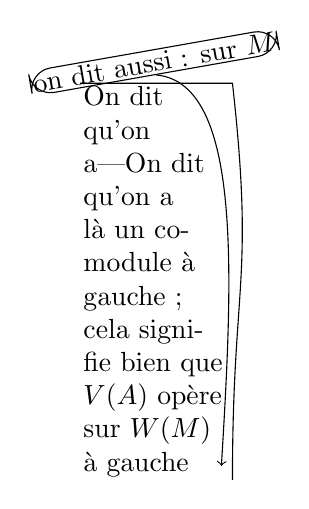
\begin{tikzpicture}[baseline=(m.base)]
 \node[align=left,text width=1.85cm,inner sep=1pt] (m) {\unsure{On dit qu'on a|On dit qu'on a là} un \unsure{comodule} à \uline{gauche} ; cela signifie \unsure{bien} que $V(A)$ opère sur $W(M)$ à gauche};
 \node[draw,rounded corners=8pt,align=center,inner sep=1pt,rotate=10,anchor=south] (g) at ([yshift=3pt]m.north) {\inserted{on dit aussi : sur $M$}};
 \draw[thin] (m.north west) .. controls ([xshift=5pt]m.north west) and (m.north) .. (m.north east) .. controls ([xshift=8pt]m.east) and (m.east) .. (m.south east);
 \draw[->,thin] (g.south) .. controls ([xshift=4pt]m.north east) and (m.east) .. ([xshift=-4pt,yshift=5pt]m.south east);
\end{tikzpicture}}
% loc 26–28, bottom lines
\deleted{loi de} l'accouplement est unitaire sss le diagramme \tikz[baseline=(t.base)]{\node[draw,circle,inner sep=1pt](t){$1'$};} comm. ; \deleted{Si $A$ muni d'une} \inserted{Elle satisfait} $\mu(\lambda x)=(\lambda\mu)x$ (ass.) sss le diagramme $2'$ est commutatif.
% archive sheet number: 25
\scanpage{27}
% loc 1–4, Soit donc A
\deleted{\unsure{Soit|Si}}Soit donc $A$ une coalgèbre (ass, \unsure{unit|unit.}) et $M$ un comodule \inserted{à g.} sur la coalgèbre. $\check A=\unsure{V|\mathbb V|W}(A)(k)$ opère à droite sur $V(M)$, donc à gauche sur $\unsure{W|V}(M)$, ou ce qui revient au $=$, sur $M$, donc \deleted{\unsure{$W($}}$M$) devient une $\check A$-\deleted{\unsure{alg}}module. Si
% loc 5–7, xi and its action
\[
\begin{aligned}
 &\xi:A\longrightarrow k\qquad(k\text{-}\mathrm{lin})\qquad\in\check A,\ x\unsure{\in|\vdash}M\\
 &\text{on a}\qquad \xi\,.\,x=(\mathrm{id}_{\unsure{M|\mu}}\otimes\xi)(u_0(x))\\
 &\text{i.e.}\qquad \xi_M=(\mathrm{id}_M\otimes\xi)\circ u_0
\end{aligned}
\]
% loc 8–10, Notons and two Hom identifications
Notons que si $\deleted{\unsure{M}}A$ est \deleted{\illegible{1} \unsure{,} \unsure{sur tout|sur tous}}\inserted{projectif de t.f. sur $k$}, on a un isom
\[
\begin{aligned}
 &\deleted{M\otimes A\simeq\mathrm{Hom}\,\mathrm{cont}_k(}\\
 &M\otimes A\simeq\mathrm{Hom}_k(\check A,M)
\end{aligned}
\]
% loc 11–13, bracketed u0 and equivalence
donc la donnée de
\tikz[baseline=(h.base)]{\node[inner sep=2pt](h){$M\overset{u_0}{\longrightarrow}M\otimes_k A$};\draw (h.south west) .. controls +(-.3,0) and +(-.12,-.15) .. (h.north west) -- (h.north east) .. controls +(-.025,-.2) and +(-.1,-.35) .. (h.south east);}
[satisfaisant certaines conditions) \deleted{\unsure{revient}}\inserted{\uline{équivaut}} à la donnée de
\[
 \check A\longrightarrow\mathrm{Hom}_k(M,M)
\]
% loc 14–18, satisfying conditions, Le = argument
satisfaisant aux conditions précédentes. On trouve alors que la donnée d'une structure de \inserted{$A$-}comodule \deleted{\unsure{équivaut à}} sur $M$. Le $=$ argument nous montre que sur le $k$-module $A$ projectif de t.f. $A$, la donnée d'une structure de coalgèbre (ass. \unsure{unit.|un?.}) équivaut à celle d'une str. d'algèbre (ass. unit.) sur $\check A$.

% loc 19–20, cancelled starts and interlinear replacements
\deleted{Si $k$ est un corps}, On a un \unsure{rsult.|résult.|résultat} analogue \deleted{\unsure{sans supposer}}\inserted{si $A$ est libre}, \deleted{\unsure{$A$ de t.f., alors}} \inserted{p.ex. $k$ un corps} ; plus 
% loc 20–23, left margin and struck limit argument
% slanted
\margin{gén. si $A$ est somme \unsure{directe} de modules \unsure{proj.} de t.f.}
\deleted{\unsure{$A$ de t.f.} En effet, \unsure{on aura} $A=\underset{\longrightarrow}{\lim}_{\unsure{i|1}}\unsure{A_i|A'}$, \unsure{$A_i$|$A'$} les sous-modules de dim finie, donc $\check A=\underset{\longleftarrow}{\lim}\unsure{A_i|A_i'|A'}$ (\unsure{lim. proj. de} \unsure{duals|duels|produits} de \unsure{vectoriels|vecteurs} de dim finie) de $\check A$}
% loc 23–26, convergence and Hom isomorphisms
Munissant $\check A$ de la topologie de la convergence simple, on aura
\[
 M\otimes_k A\simeq\mathrm{Hom}\,\mathrm{cont}_k(\check A,M)
\]
donc
\[
 \mathrm{Hom}(\unsure{N|W},M\otimes_{\unsure{k|u}}A)
 \simeq\mathrm{Hom}\,\mathrm{cont}_{\unsure{K|k}}\bigl(\check A,\,
 \underbrace{\deleted{\unsure{H}}\mathrm{Hom}_k(N,M)}_{\substack{\text{muni de}\\\text{la top. de la}\\\text{conv. simple}}}\bigr)
\]
% loc 27–28, sentence continuing on scan 28
donc on trouve qu'une structure de \unsure{comodule} (\unsure{ass.} unit) sur $M$ revient à la donnée d'un
% archive sheet number: 26
\scanpage{28}
% loc 1–3, continuation at upper edge
structure de $\unsure{\widetilde A|\check A}$-module sur $M$ tel que pour \unsure{tt|tout} $x\in M$, $\xi\longmapsto\xi x$ soit continue (i.e. s'annule sur un des $J_{\unsure{i|1|\prime}}\subset\check A\ \ldotp\ldotp\ldotp\ldotp\ \unsure{]|\exists}$. 
% loc 3–6, De =, on voit
De $=$, on voit que la donnée \deleted{\unsure{s}}d'une structure de coalgèbre \inserted{(\unsure{ass. unit})} sur le $k$-module libre $A$ revient à la donnée d'une \deleted{opération} structure de $k$-algèbre (ass. unitaire) sur $\check A$ qui soit \uline{continue}
% loc 7–8, car si; struck line and formula
[car si $\overset{\inserted{\unsure{k^{I}}}}{\overset{\scriptscriptstyle\unsure{\tikz[baseline=-.4ex]{\node[rotate=90,inner sep=0pt]{\(\scriptscriptstyle\simeq\)};}|\Vert}}{P}},\overset{\inserted{\unsure{k^{J}}}}{\overset{\tikz[baseline=-.4ex]{\node[rotate=90,inner sep=0pt]{\(\scriptscriptstyle\simeq\)};}}{Q}},\overset{\inserted{\unsure{k^{\Lambda}}}}{\overset{\scriptscriptstyle\Vert}{R}}$ sont libres, \deleted{les \unsure{accouplements|applications} \inserted{bil.} continus $\check P\times\check Q\unsure{\longrightarrow|-}\check R=\underset{\leftarrow}{\lim}_{\unsure{\alpha|\lambda}}\deleted{\unsure{R_{I}}}R_{\unsure{\Lambda_{\alpha}|\Lambda_2}}$.}
% loc 9–16, multiline Bil and Hom display
\[
\begin{aligned}
\unsure{\mathrm{bil}|\mathrm{Bil}}\,\mathrm{cont}_{k}\,\check P,\check Q;\check R)
 &\simeq \mathrm{Bil}\,\mathrm{cont}_{k}(\check P,\check Q;\underset{\leftarrow}{\lim}_{\gamma}(\check R_{\gamma}))\\
 &\simeq \underset{\leftarrow}{\lim}_{\gamma}\,[\mathrm{bil}\,\mathrm{cont}_{k}(\check P,\check Q;\check R_{\gamma})]\\
 &\simeq \underset{\leftarrow}{\lim}_{\gamma}\,\bigl[\underset{\unsure{\rightarrow|-}}{\lim}_{\alpha,\beta}\,
 \underbrace{\mathrm{Bil}_{k}(\check P_{\alpha},\check Q_{\beta};\check R_{\gamma})}_{\mathrm{Hom}_{k}(\check P_{\alpha}\otimes\check Q_{\beta};\check R_{\gamma})\,]}\bigr]\\
 &\deleted{\unsure{\simeq}}\\
 &\simeq \underset{\leftarrow}{\lim}_{\gamma}\,\underset{\rightarrow}{\lim}_{\alpha,\beta}\,\mathrm{Hom}_{k}(R_{\gamma},P_{\alpha}\otimes Q_{\beta})\\
 &\simeq \underset{\leftarrow}{\lim}_{\gamma}\,\mathrm{Hom}_{k}(R_{\gamma},P\otimes Q)\\
 &\simeq \mathrm{Hom}_{k}(R,P\otimes Q)\qquad !\quad ]
\end{aligned}
\]

% loc 17–21, On est dans
\deleted{On a également le même résultat} \inserted{On est dans le cas envisagé} si $A$ est limite \deleted{\unsure{projective}}\unsure{inductive} \uline{dénombrable} de sous-modules projectifs \inserted{de t.f.}, à morphismes de transition \deleted{ayant} des \deleted{suppléments} mon. \unsure{univ.|inv.} [i.e. ayant des inverses à g.] Mais dans le cas général, on ne peut oublier $V(A)$ \inserted{et ses opérations} au profit de $\check A=V(A)(k)$ $\ldots$

% loc 22–27, Module quotient and quotient map
Module quotient et sous-module stable par une co-opération de la co-algèbre $A$ : Soit $M\overset{\unsure{g|f}}{\unsure{\longrightarrow|-}}N'$ un ép., alors $V(N)\subset V(M)$ mono, et il est clair ce que signifie que $V(N)$ est stable ; on dira alors que $N$ est stable par la coop. de $N$. \unsure{Cel|Cela} signifie aussi que $\exists$ un hom $N'\overset{\omega_{N'}}{\longrightarrow}N'\otimes A$ rendant comm.
% loc 27–28, commutative square
\diagram{\begin{tikzcd}[ampersand replacement=\&,column sep=large]
M\arrow[r,"\omega_M"]\arrow[d] \& M\otimes A\arrow[d,"g\otimes\mathrm{id}_{A}"]\\
N'\arrow[r,"\omega_{N'}"] \& N'\otimes A
\end{tikzcd}}
% loc 29–30, last two lines
et cet $\omega_{N}$ est néc. unique et satisfait aux axiomes d'unité et associativité. Si $A$ est \unsure{un gp.|une alg.|var.} affine
% archive sheet number: 27
